\documentclass[
  paper=a4,
  titlepage,
  bibliography=totoc,
  listof=totoc,
  pagesize=pdftex
]{scrartcl}
% TMP
\overfullrule=1mm
% TMP
\usepackage[utf8]{inputenc}
\usepackage[T1]{fontenc}
\usepackage[english]{babel}
\usepackage[autostyle=true]{csquotes}
\usepackage{enumitem}
\usepackage{mathtools,amsfonts,amssymb,amsthm,mathrsfs}
\usepackage{lmodern}
\usepackage{dsfont}

\usepackage[noend]{algpseudocode}
\algrenewcommand\algorithmicrequire{\textbf{Input:}}
\algrenewcommand\algorithmicensure{\textbf{Output:}}

\usepackage[
  activate={true,nocompatibility},
  kerning=true,
  spacing=true
]{microtype}

\usepackage{pgf,tikz}
\usetikzlibrary{calc}
\usepackage[pdftex,hidelinks]{hyperref}

\usepackage[
  backend=biber,
  style=alphabetic,
  maxnames=10,
  maxalphanames=5,
  isbn=false
]{biblatex}
\addbibresource{bachelor.bib}

% serif > sans-serif
\setkomafont{sectioning}{\rmfamily\bfseries\boldmath}
\setkomafont{descriptionlabel}{\rmfamily\bfseries\boldmath}
% prefix all numbers with section
\numberwithin{figure}{section}
\numberwithin{equation}{section}
\numberwithin{table}{section}

% set default numbered list style to (i), (ii), ...
\setlist[enumerate,1]{label=(\roman*)}

% use mathds instead of mathbb
\newcommand*\setZ{\mathds{Z}}
\newcommand*\setR{\mathds{R}}
\newcommand*\setC{\mathds{C}}
\newcommand*\setQ{\mathds{Q}}
\newcommand*\setN{\mathds{N}}
\newcommand*\setK{\mathds{K}}
\newcommand*\setA{\mathds{A}}
\newcommand*\setP{\mathds{P}}
\newcommand*\setT{\mathds{T}}
\newcommand*\ii{\mathrm{i}}

% number a single equation in unnumbered environment
\newcommand\numberthis{\addtocounter{equation}{1}\tag{\theequation}}
\newcommand*\dotcup{\mathbin{\dot{\cup}}}

% shorthands
\newcommand*\ideal[1]{\left\langle #1 \right\rangle}
\newcommand*\puiseux[2]{#1\{\!\{#2\}\!\}}
\newcommand*\CCt{\puiseux{\setC}{t}}

\let\vec\mathbf
\let\idealof\trianglelefteq

% operators
\DeclareMathOperator{\Mat}{Mat}
\DeclareMathOperator{\lcm}{lcm}
\DeclareMathOperator{\Trop}{Trop}
\DeclareMathOperator{\trop}{trop}
\DeclareMathOperator{\initial}{in}
\DeclareMathOperator{\face}{face}
\DeclareMathOperator{\GF}{GF}
\DeclareMathOperator{\GR}{GR}
\DeclareMathOperator{\conv}{conv}
\DeclareMathOperator{\Lin}{Lin}
\DeclareMathOperator{\codim}{codim}

% use same counters for all environments
\theoremstyle{definition}
\newtheorem{definition}{Definition}
\newtheorem{theorem}[definition]{Theorem}
\newtheorem{proposition}[definition]{Proposition}
\newtheorem{example}[definition]{Example}
\newtheorem{remark}[definition]{Remark}
\newtheorem{lemma}[definition]{Lemma}
\newtheorem{algo}[definition]{Algorithm}
\newtheorem{thmCorollary}[definition]{Theorem \& Corollaries}

% adjust numbering
\numberwithin{definition}{section}

\title{Massively Parallel Computation of Tropical Varieties}
\subtitle{Bachelor's Thesis}
\author{Dominik Bendle}
\publishers{supervised by Janko Böhm,\\TU Kaiserslautern}
\date{\today}

\begin{document}
\pagestyle{headings}

\maketitle

\tableofcontents
\newpage

\section{Overview}

Give general introduction to topic

Describe work done at ITWM and their assistance

Mention $\mathcal G_{3,8}$ which has not been computed prior and give some properties of the
fan.

Work exposed several memory leaks and small errors in \textsc{Singular} kernel, were able
to be fixed.

Our results are implemented in computer algebra system \textsc{Singular} \cite{Singular}
with parallelization work done using GPI-Space at the ITWM.

% TODO more motivation

In the second section we will introduce the basic concepts of tropical geometry and
tropical varieties. We will discuss several different approaches of computing tropical
varieties, including considering the Gröbner fan of an ideal and the new Newton polygon
method described in \cite{tropPointsLinks}. Consequently we will take a look at Puiseux
series rings which are special fields with valuation and fundamental to our results. In
the third section we describe Petri nets as a language to formulate parallelizable
workflows.

% TODO more here

\section{Computing Tropical Varieties}

Tropical geometry is a relatively new field in mathematics that arises from numerous
contexts and connects various branches of mathematics in exciting and novel ways. We shall
provide a basic introduction to this topic while focusing on the computational aspects
which will lead to the main interest of this thesis -- the recently developed techniques
using Newton polygons and valuations.

Over the course of this section we need some basic definitions from algebraic geometry: We
fix a field $K$ which is usually assumed to be algebraically closed: The \emph{affine
space} over $K$ of dimension $n$ is
\[
  \setA_K^n = \setA^n = \left\{ (a_1,\dots,a_n) : a_i \in K\right\} = K^n
\]
and the \emph{projective space} over $K$ of dimension $n$ is $\setP^n_K = \setP^n =
(K^{n+1}\setminus\{0\})/\sim$ with equivalence relation $v \sim \lambda v$ for all $v \in
K^n\setminus \{0\}$ and $\lambda \in K^*$. Elements $a \in \setP^n$ are usually written as
homogeneous coordinates $(a_1:\cdots:a_n)$ for a representative $(a_0, \dots, a_n)$. An
\emph{affine variety} is the common zero locus of all the polynomials of a polynomial
ideal $I \idealof K[x_1, \dots, x_n]$, that means sets of the form
\[
  X := V(I) = \{ a \in \setA^n : f(a) = 0 \text{ for all $f\in I$} \} \subset \setA^n.
\]
In the special case of a homogeneous ideal $I \idealof K[x_0,\dots,x_n]$, which means $I$
is generated by homogeneous polynomials -- we may define \emph{projective varieties}
\[
  X := V(I) = \left\{ (a_0:\cdots:a_n) \in \setP^n : f(a_0, \dots, a_n) = 0
    \text{ for all $f \in I$}
  \right\} \subset \setP^n.
\]
The homogeneity assumption is necessary since otherwise $f(a)$ being zero is not
independent from the representative $a$ of $a\in \setP^n$.

\subsection{Basic Tropical Geometry}
\label{sec:tropIntro}

The standard approach to tropical geometry is to consider the semiring $(\setR \cup
\{\infty\}, \min, +)$ with the classical addition replaced with taking the minimum and
classical multiplication replaced with addition. An in-depth introduction to tropical
geometry and tropical varieties is given by \cite{sturmMacTrop}, similar notions focused
on computation can be found in \cite{compTropVar}.

We denote by $\oplus$ and $\odot$ the \enquote{addition} and \enquote{multiplication}
defined above, so -- just to reiterate -- we have that
\[
  x \oplus y = \min(x,y)
  \qquad \text{and} \qquad
  x \odot y = x+y
\]
for elements $x,y\in \setR\cup\{\infty\}$, for example $4\oplus9 = 4$ and $4\odot9 = 13$.
It is easy to verify that the usual arithmetic laws are still valid: $\oplus$ and $\odot$
are commutative and satisfy distributivity. Further, there is a unique neutral  element
for both operations: For all $x\in \setR\cup \{\infty\}$ it is true that
\[
  x \oplus \infty = x
  \qquad \text{and} \qquad
  x \odot 0 = x.
\]
As in proper rings, the neutral element of $\oplus$ has the annihilating property with
respect to $\odot$, i.e.\ $x\odot \infty = \infty$. An important property of this set is
that, while elements in $\setR$ admit a multiplicative $\odot$-inverse (the traditional
additive inverse), there is in general no additive $\oplus$-inverse. For example the
equation $4\oplus x = 5$ clearly has no solution. In this setting all ring axioms except
the existence of an additive inverse are satisfied: Sets like this are in fact called
semirings, hence we call $(\setR\cup \{\infty\}, \oplus, \odot)$ the \emph{tropical
semiring} which is sometimes also referred to a as the \emph{min-plus algebra}. By
replacing taking minima with maxima, we obtain the isomorphic max-plus algebra which is
also used as the underlying structure in tropical geometry by some authors. These special
operations of addition and multiplication naturally lead to the notion of polynomials over
the tropical semiring.

\begin{definition}[Tropical Polynomials]
  \label{def:tropPoly}
  Let $x_1, \dots, x_k$ be variables with values in $\setR\cup\{\infty\}$, then due to
  commutativity we can write arbitrary products of variables as
  \[
    x_{i_1} \odot x_{i_2} \odot \cdots \odot x_{i_m}
    = x_1^{\alpha_1} \cdots x_k^{\alpha_k}
  \]
  for suitable $\alpha_1, \dots, \alpha_k \in \setN$. Unsurprisingly we call this a
  \emph{tropical monomial}. Translating back into the traditional operations shows that
  the tropical monomials
  \[
    x_1^{\alpha_1} \cdots x_k^{\alpha_k} =
    \underbrace{x_1\odot\cdots\odot x_1}_{\alpha_1 \text{ times}}
    \odot\cdots\odot
    \underbrace{x_k\odot\cdots\odot x_k}_{\alpha_k \text{ times}}
    = \alpha_1x_1 + \cdots + \alpha_kx_k
  \]
  are just linear polynomials with integer coefficients. A \emph{tropical polynomial} is
  then defined as a finite $\setR$-linear combination of tropical monomials with respect
  to tropical arithmetic:
  \[
    p = a_1 \odot x_1^{\alpha_{1,1}}\cdots x_k^{\alpha_{1,k}} \oplus \cdots \oplus
    a_m \odot x_1^{\alpha_{m,1}}\cdots x_k^{\alpha_{m,k}}
  \]
  with exponents $\alpha_{i,j} \in \setN$, $1\leq i \leq m, 1\leq j \leq k$ and real
  coefficients $a_i \in \setR$. Note that if $a_i = 0$ for some $i$ we have that $a_i\odot
  x_1^{\alpha_{i,1}}\cdots x_k^{\alpha_{i,k}} = x_1^{\alpha_{i,1}}\cdots
  x_k^{\alpha_{i,k}}$ so we can omit $0$-coefficients. As usual, we call a monomial in $p$
  together with its coefficient a \emph{term}.
\end{definition}

\begin{figure}[tbh]
  \centering
  \begin{tikzpicture}
    \draw[->] (-0.1,0) -- (5.5,0) node[right] {$x$};
    \draw[->] (0,-0.1) -- (0,5.5) node[left] {$p(x)$};
    \begin{scriptsize}
      \foreach \x in {1, 2, 3, 4, 5}
      {
        \draw (0.1,\x) -- (-0.1,\x) node[left] {$\x$};
        \draw (\x,0.1) -- (\x,-0.1) node[below] {$\x$};
      }
    \end{scriptsize}

    \draw[dashed] (-0.05,-0.1) -- (2.75,5.5);
    \draw[dashed] (-0.1,1.9) -- (3.5,5.5);
    \draw[dashed] (-0.1,5) -- (5.5,5);
    \draw[thick] (-0.05,-0.1) -- (2,4) -- (3,5) -- (5.5,5);
  \end{tikzpicture}
  \caption{Graph of the tropical polynomial $p=x^2\oplus 2\odot x \oplus 5$}
  \label{fig:tropPolyPlot}
\end{figure}

By again translating back to the traditional operations, evaluating this polynomial at
elements in $\setR^k$ yields a function
\[
  p : \setR^k \to \setR, (x_1, \dots, x_k) \mapsto
  \min\left\{
    a_i + \sum_{j=1}^k \alpha_{i,j}x_j : 1 \leq i \leq m
  \right\}
\]
which is continuous, piecewise linear with finitely many pieces and concave, meaning that
for any $a,b \in \setR^k$ the equality $p(\frac12(a+b)) \geq \frac12(p(a)+p(a))$ holds.
Consider for example the polynomial $p = x^2 \oplus 2\odot x \oplus 5$ in the single
variable $x$. As we see in figure~\ref{fig:tropPolyPlot}, each monomial of $p$ corresponds
to a linear piece of the graph and the function $p$ is in fact concave.

With the newly established notion of tropical polynomials the next step towards defining
tropical varieties is to consider special sets $X \subset \setR^k$ induced by a tropical
polynomial. Whereas the main object of study in classical algebraic geometry are the roots
or vanishing loci of polynomials and -- by extension -- polynomial ideals, being zero is
not a particularly interesting property of a tropical polynomial. Similarly, evaluating to
the additive identity is equally uninteresting: If $p$ is not already the constant
$\infty$-function, then $p(x)=\infty$ if and only if $x=\infty$. Instead, we use the fact
that the induced function is piecewise linear:

\begin{definition}[Tropical Hypersurface]
  \label{def:tropHypersurface}
  Let $p = \bigoplus_{i=1}^k a_i \odot x_1^{\alpha_{i,1}}\cdots x_k^{\alpha_{i,k}}$ be a
  tropical polynomial in the variables $x_1, \dots, x_k$ with induced piecewise linear
  function $p:\setR^k \to \setR$. For an element $a\in \setR^k$ the value $p(a)$ is the
  minimum over the terms of $p$; we set
  \[
    V(p) = \left\{
      a \in \setR^k :
      \text{ the minimum $p(a)$ is attained by at least two terms of $p$}
    \right\}
  \]
  and call it the \emph{tropical hypersurface} of $p$. Equivalently, a point $a\in
  \setR^k$ lies in $V(p)$ if and only if $p$ is not linear at $a$. With this
  interpretation in mind, the set $V(p)$ is also called the \emph{corner locus} of $p$.
\end{definition}

Again looking at the tropical polynomial $p$ plotted in figure~\ref{fig:tropPolyPlot} we
see that $p$ is not linear at precisely the points $V(p) = \{ 2, 3 \}$. An interesting
property is that by this definition the tropical hypersurface given by a monomial contains
no points whatsoever. This will become important later on.

\begin{figure}[tbh]
  \centering
  \begin{tikzpicture}[thick]
    \draw (0,0) -- (2,2);
    \draw (2,2) -- (2,4.5);
    \draw (2,2) -- (4.5,2);
  \end{tikzpicture}
  and quadric
  % TODO
  \caption{A generic tropical line and quadric in $\setR^2$}
  \label{fig:tropLineQuad}
\end{figure}

Since monomials and powers of variables are well-defined, we can assign a \emph{degree} to
a tropical polynomial in the usual sense, hence we may carry over the naming conventions
for hypersurfaces in standard algebraic geometry: A hypersurface given by a degree 1
polynomial is called a tropical hyperplane, for degrees 2, 3 and so on they are called
tropical quadrics and cubics respectively. In figure~\ref{fig:tropLineQuad} we see the
hypersurfaces given by \dots % TODO
As a final note, since tropical division is well-defined for non-infinite elements we may
also consider tropical polynomials in negative exponents later on.

\subsection{Valuations and Puiseux Series}

Most of the following definitions and algorithms will make use of fields equipped with a
non-trivial valuation: We fix a field $K$ and recall that a \emph{valuation} is a map
$\nu:K\to \setR \cup \{\infty\}$ that satisfies the following properties: For any $a, b
\in K$ we have
\begin{enumerate}
  \item $\nu(a) = \infty$ if and only if $a=0$,
  \item $\nu(ab) = \nu(a)+\nu(b)$ and
  \item $\nu(a+b) \geq \min\{\nu(a), \nu(b)\}$ with equality if $a\neq b$.
\end{enumerate}
A valuation is called \emph{non-trivial} if it is not the constant 0-function on $K^* =
K\setminus\{0\}$. Such a field with valuation defines a local ring $R_\nu = \{ x \in K :
\nu(x) \geq 0 \}$ with unique maximal ideal $\mathfrak m_{R_\nu} = \{ x \in K : \nu(x) > 0
\}$. The \emph{residue field} of $K$ is then defined to be the residue field $\mathfrak K
= R_\nu/\mathfrak m_{R_\nu}$ of $R_\nu$. Any generator $t \in R_\nu$ of $\mathfrak
m_{R_\nu}$ is called a \emph{uniformizing parameter}.

While there are various fields admitting a non-trivial valuation that
are suitable for tropical computations, the most important one for our case is the field
of Puiseux series:

\begin{definition}[Puiseux Series]
  \label{def:puiseux}
  Let $K'$ be a field. The field of \emph{Puiseux series} $K = \puiseux{K'}{t}$ with
  coefficients in $K'$ in the indeterminate $t$ is the set of all formal power series
  \begin{equation} \label{eq:puiseux1}
    f = c_1 t^{a_1} + c_2 t^{a_2} + c_3 t^{a_3} + \cdots
  \end{equation}
  with $c_k \in K'$ for all $k \in \setN$ and rational numbers $a_1 < a_2 < a_3 < \cdots$
  that have a common denominator. Hence, the series can be rewritten as
  \begin{equation} \label{eq:puiseux2}
    f = \sum_{k = k_0}^\infty c'_k t^{\frac kN}
  \end{equation}
  with suitable $c'_k \in K'$ for all $k\geq k_0$, $c_{k_0}\neq0$ and the common
  denominator $N \in \setN$.
\end{definition}

By considering the rings of formal Laurent series $\smash{K'((t^{\frac1n}))}$ for $n \in
\setN$ in the indeterminate $\smash{t^{\frac1n}}$, we can see that
\[
  K = \puiseux{K'}t = \bigcup_{n \in \setN} K'((t^{\frac1n})).
\]
The most important use case will involve $K'$ being algebraically closed, in particular we
usually choose $K'=\setC$. This is due to the following theorem:

\begin{theorem}
  \label{thm:puisuexalgclosed}
  If $K'$ is an algebraically closed field of characteristic 0, then $K :=
  \puiseux{K'}{t}$ is also algebraically closed. In particular, $K$ is the algebraic
  closure of the field of formal Laurent series $K'((t))$.
\end{theorem}

The proof of this theorem is constructive and -- provided one can compute roots over the
base field $K'$ -- yields a method to iteratively compute roots of a polynomial in
$\puiseux{K'}{t}[x]$ up to a given order, see for example the proof of
\cite[Theorem~2.1.5]{sturmMacTrop}. As we will see, finite \emph{expansions} of these
roots will more than suffice for our purposes. The proof cited above uses the natural
valuation $\nu : \puiseux{K'}{t} \to \setR \cup \{\infty\}$ of this field: for an element
$f \in \puiseux{K'}{t}^*$ we define $\nu(f)$ to be the lowest exponent that appears in a
non-zero term of $f$, i.e.\ $a_1$ in \eqref{eq:puiseux1} and $k_0/N$ in
\eqref{eq:puiseux2}.

\begin{example}
  Let $L$ be any field and fix $K' = \setC$ so $K = \CCt$.
  \begin{enumerate}
    \item If we equip $L$ with the trivial valuation $\nu(K^*) = \{0\}$, then we have
      $R_\nu = K$ and $\mathfrak m_{R_\nu} = \{0\}$, so $\mathfrak K = K$.
    \item By the definitions it is clear that the residue of the Puiseux series ring
      $\CCt$ must be $\mathfrak K = \setC$. % TODO
    \item The Puiseux series $t^{\frac12}, t^{\frac12} + t^{\frac23} + t^2,
      \sum_{i=1}^\infty \frac1i t^{\frac i2} \in \CCt$ all have valuation $\frac12$.
    \item % TODO
    \item We will come back to computing computing finite expansions of roots of
      univariate polynomials in a later section, see
      Example~\ref{ex:zeroDimTrop}.\ref{ex:zdt2}.
  \end{enumerate}
\end{example}

\dots % TODO

% also need this
\begin{lemma}[{\cite[Lemma~2.1.15]{sturmMacTrop}}]
  \label{lem:valSplit}
  Denote the valuation group of $\nu$ by $\Gamma_\nu = \nu(K^*)$. If $K$ is algebraically
  closed, then there is a group homomorphism $\psi : \Gamma_\nu \to K^*$ with
  $\nu(\psi(w)) = w$ for all $w \in \Gamma_\nu$. In other words, the surjection $\nu : K^*
  \to \Gamma_\nu$ splits.
\end{lemma}

We will use the notation $t^w$ for the elements $\phi(w) \in K^*$ which is motivated by
the most important field for our purposes: In the case $K = \CCt$ we have $\Gamma_\nu =
\setQ$ and the element $t^w$ will be exactly this power of $t$.

While working in polynomial rings over $\CCt$ or similar fields with valuation mainly
provides theoretical benefits like using Newton polygons to determine valuations of roots
as in Lemma~\ref{lem:newtPolyRoots}, the iterative method given by
Theorem~\ref{thm:puisuexalgclosed} will provide a fall-back method of computing
zero-dimensional affine varieties. To this end we usually consider elements of $\setQ(t)$
as finite approximations of Puiseux series.
% mention Santiagos work here?

\subsection{Gröbner Fans}
\label{sec:grobFan}

One way of looking at the tropical variety of a polynomial ideal $I \idealof K[\vec x] :=
K[x_1, \dots, x_n]$ is to first consider its Gröbner fan. This fan partitions the space
$\setR^n$ into polyhedral cones which contain all weight vectors $w\in \setR^n$ that
define the same initial ideal of $I$. While this fan is a highly interesting object of
study in and on itself, by restricting the fan to those cones which correspond to
monomial-free initial ideals, we obtain the tropical variety of the given ideal.

We start off this section with some basic definitions from convex geometry which will lead
to the definition of the Gröbner fan of an ideal. This will then allow us to define
tropical varieties and demonstrate their connection to the Gröbner fan. For this we mainly
focus on definitions and results found in \cite{compGrobFan} and \cite{SturmGBCP}. The
first step towards defining a fan is to understand the very important concept of polyhedra
and polyhedral cones:

\begin{definition}[Polyhedral Cones]
  \label{def:polyhedralCone}
  Recall that a set of the form $C = \{ \vec x \in \setR^n : A\vec x \leq \vec b \}$ for
  some matrix $A \in \Mat(m\times n, \setR)$ and $\vec b \in \setR^m$ is called a
  polyhedron and if additionally $C$ is bounded it is called a polytope. If on the other
  hand $\vec b=0$ then $C$ is called a \emph{polyhedral cone}. Equivalently, a polyhedral
  cone $C$ is the positive span of finitely many vectors in $\setR^n$.
\end{definition}

Note that, using Linear Programming, it is possible to assign a unique \emph{canonical}
set of defining equations to a polyhedral cone. This is important to quickly compare and
uniquely identify polyhedral cones, especially in computational contexts.

For a polyhedron $P \subseteq \setR^n$ we further define its dimension as the dimension of
the smallest affine linear space containing $P$. Consider now an element $\vec w \in
\setR^n$, then we define the set $\face_{\vec w}(P) = \{ \vec u \in P : \vec w\cdot \vec u
\geq \vec w \cdot \vec v \text{ for all } \vec v\in P\}$ where the vector multiplication
is the standard scalar product on $\setR^n$. Surprisingly enough, we call a subset of $P$
of the form $\varnothing$ or $\face_{\vec w}(P)$ a \emph{face} of $P$. For example, the
trivial faces of $P$ are $\varnothing$ by definition and $P = \face_{\vec 0}(P)$. Clearly,
a face of $P$ is a polyhedron itself, so we call it a facet if it has dimension exactly
one less than $P$. The notion of faces is important for the next definition:

\begin{definition}[Polyhedral Fan]
  \label{def:polyhedralFan}
  Let $\mathcal C$ be a collection of polyhedra in $\setR^n$. We call $\mathcal C$ a
  \emph{polyhedral complex} if
  \begin{enumerate}
    \item all non-empty faces of $P$ are in $\mathcal C$ for all $P \in \mathcal C$ and
    \item for any $P,Q \in \mathcal C$ the intersection $P\cap Q$ is a face of both $P$
      and $Q$.
  \end{enumerate}
  The support of $\mathcal C$ is $\bigcup_{P\in\mathcal C}P$ and we call $\mathcal C$ a
  \emph{polyhedral fan} if all polyhedra in $C$ are polyhedral cones. Furthermore, if the
  support of a polyhedral fan is all of $\setR^n$ we call it \emph{complete}.
\end{definition}

Intuitively, a polyhedral complex is a collection of polyhedra where intersecting
arbitrary elements does not produce new polyhedra and -- more importantly -- if the
intersection of two such polyhedra is a non-trivial face of both of them, they only
\enquote{touch}. To make polyhedral complexes easier to work with we call a collection of
polyhedra a \emph{representation} of a complex $\mathcal C$ if each polyhedron $P \in
\mathcal C$ is a face of some $S \in \mathcal S$. In particular, the maximal polyhedra of
a polyhedral complex define a representation.

Now, given a polynomial ring $K[\vec x]$ a total \emph{term} or \emph{monomial ordering}
$\prec$ on the monomials $K[\vec x]$ is an ordering such that $1 \prec \vec x^\alpha =
x_1^{\alpha_1}\cdots x_n^{\alpha_n}$ for all $\alpha \in \setN^n$ and if $\vec x^\alpha
\prec \vec x^\beta$ for some $\alpha, \beta \in \setN^n$ then also $\vec x^{\alpha+\gamma}
\prec \vec x^{\beta+\gamma}$ for all $\gamma \in \setN^n$. Hence we can order the non-zero
terms of any non-zero polynomial $f \in K[\vec x]$ which defines a unique maximal
\emph{initial term} $\initial_\prec(f)$. Correspondingly, for an ideal $I \idealof K[\vec
x]$ we define the \emph{initial ideal} of $I$ as $\initial_\prec(I) = \ideal{\initial_\prec(f)
: f \in I}$. Initial ideals are used to define one of the most important concepts in
computer algebra: A finite subset $\mathcal G \subset I$ is called a \emph{Gröbner basis}
of the ideal $I$ with respect to $\prec$ if its initial terms $\mathcal G' = \{
\initial_\prec(g) : g \in \mathcal G \}$ generate $\initial_\prec(I)$. Further, if the
elements of $\mathcal G'$ are irredundant $\mathcal G$ is called \emph{minimal} and if for
any $g, g' \in \mathcal G$ no terms of $g$ are divisible by $\initial_\prec(g')$ then
$\mathcal G$ is \emph{reduced}. The reduced Gröbner basis of an ideal $I$ with respect to
$\prec$ can be shown to be unique up to scaling with units, so we denote it by $\mathcal
G_\prec(I)$. While there are infinitely many possible term orderings in polynomial rings
with more than one variable, one can show that for a fixed $I \idealof K[\vec x]$ there
are only finitely many different initial ideals using the Noetherian property of
polynomial rings over fields.

Using this argument we are interested in grouping all term orderings into finitely many
classes, but this first requires a way to identify a given ordering with a more tangible
description. The idea is to represent term orderings by weight vectors:

\begin{definition}[Initial Forms]
  \label{def:initFormG}
  Given a $\vec w \in \setR^n$ we define the \emph{initial form} $\initial_{\vec w}(f)$ of
  $f = \sum_{\alpha\in\setN^n} c_\alpha \vec x^\alpha \in K[\vec x]$ with respect to $\vec
  w$ to be the sum of all non-zero terms $c_\alpha \vec x^\alpha$ of $f$ where $\vec
  w\cdot \alpha$ is maximal. Analogously to initial terms this defines an initial ideal
  $\initial_{\vec w}(I)$ for $I \idealof K[\vec x]$.
\end{definition}

Note that initial ideals of this form need not be monomial ideals -- in fact the weight
vectors for which this is not the case will be of interest later on. If necessary, this
can be fixed by introducing a \enquote{tie breaker} ordering: Given any total term
ordering $\prec$ and any weight vector $\vec w\in\setR^n$ with non-negative components we
may define a new term ordering $\prec_{\vec w}$ by
\[
  \vec x^\alpha \prec_{\vec w} \vec x^\beta
  \quad\iff\quad
  \vec w \cdot \alpha < \vec w\cdot \beta
  \text{ or }
  \left(
    \vec w \cdot \alpha = \vec w\cdot \beta
    \text{ and }
    \vec x^\alpha \prec \vec x^\beta
  \right)
\]
where the non-negativity constraint is required to ensure that $\prec_{\vec w}$ is also a
total ordering, meaning that 1 will be smaller than any other monomial with respect to
$\prec_{\vec w}$. Among some other nice properties, the most important result obtained
from these constructions is the following:

\begin{proposition}[{\cite[Proposition~1.11]{SturmGBCP}}]
  \label{prp:init}
  For any global term ordering $\prec$ and any ideal $I \idealof K[\vec x]$ there is a
  weight vector $\vec w \in \setR^n_{\geq0}$ with $\initial_\prec(I) = \initial_{\vec
  w}(I)$.
\end{proposition}

Hence it makes sense to only consider initial forms and ideals given by non-negative
weight vectors $\vec w \in \setR^n_{\geq0}$. The next step is to group these weight
vectors into classes: For a given $I \idealof K[\vec x]$ we call two weights $\vec w, \vec
w' \in \setR^n$ \emph{equivalent} if $\initial_{\vec w}(I) = \initial_{\vec w'}(I)$ and it
is easy to see that this indeed defines an equivalence relation. Denoting the
corresponding equivalence classes by
\[
  C[\vec w] = \left\{
    \vec w' \in \setR^n : \initial_{\vec w'}(I) = \initial_{\vec w}(I)
  \right\},
\]
In section 2 of \cite{compGrobFan} it is show that each $C[\vec w]$ is a relatively open
convex polyhedral cone if the equivalence class contains a strictly positive vector. This
immediately leads to the following definitions:

\begin{definition}[Gröbner Cones and Fans]
  \label{def:groebnerConeFan}
  Fix an ideal $I \idealof K[\vec x]$. For a weight $\vec w \in \setR^n$ with $C[\vec w]
  \cap \setR^n_{>0} \neq \varnothing$ we call the Euclidean closure $C_{\vec w}(I) :=
  \overline{C[\vec w]}$ the \emph{Gröbner cone} of $I$ with respect to $\vec w$. The
  collection of all these cones $\GF(I) := \{ C_{\vec w}(I) : \vec w \in \setR^n_{\geq0}
  \}$ is called the \emph{Gröbner fan} of $I$.
\end{definition}

% TODO change ...
In \cite[Theorem~2.19]{compGrobFan} it is shown that the Gröbner fan is in fact a fan.
Its support $\GR(I) = \{ \vec w \in \setR^n : \exists \vec w' \in
\setR^n_{\geq0}:\initial_{\vec w}(I) = \initial_{\vec w'}(I)\}$ is called the
\emph{Gröbner region} of $I$. The main source \cite{SturmGBCP} introduces Newton polytopes
as a means to compute the Gröbner fan of an ideal which work similarly to what we will
introduce in Definition~\ref{def:newtonPoly}, but no more theory is required for this
section. The connection to tropical varieties will be drawn in the next section. We may
also occasionally need Gröbner cones with respect to a given term ordering. By
Proposition~\ref{prp:init} for any $I \idealof K[\vec x]$ and term order $\prec$ there is
a $\vec w \in \setR^n_{\geq0}$ with $\initial_\prec(I) = \initial_{\vec w}(I)$. Hence we
define the corresponding Gröbner cone to be $C_\prec(I) := C_{\vec w}(I)$.

\subsection{Tropical Varieties}
\label{sec:tropVar}

After this light introduction to tropical arithmetic and some convex geometry we now shift
our focus to more general polynomials and ideals. The idea is to combine the fan structure
of tropical varieties we derived in section~\ref{sec:grobFan} with our knowledge on
tropical hypersurfaces from section~\ref{sec:tropIntro}. Here we will introduce the
general procedure of computing a tropical variety by computing cones in the corresponding
fan and finding its neighbor cones.

We fix a field $K$ which admits a usually non-trivial valuation $\nu : K \to \setR \cup
\{\infty\}$. The usual setting is to consider the \emph{Laurent polynomial} ring $K[\vec
x^{\pm1}] = K[x_1^{\pm1}, \dots, x_n^{\pm1}]$ -- the ring of polynomials in $x_1, \dots,
x_n$ with integral but not necessarily non-negative exponents. Ideals and polynomials in
this ring define zero loci much in the same manner as for standard polynomial rings,
however as monomials are now invertible, evaluation at zero is no longer well-defined. As
such, we consider the \emph{very affine variety} of an ideal $I \idealof K[\vec x^{\pm1}]$
as a subset of the \emph{algebraic torus} $\setT^n := {(K^*)}^n = {(K \setminus
\{0\})}^n$:
\[
  X := V(I) = \left\{ a \in \setT^n : f(a) = 0 \text{ for all $f \in I$} \right\}.
\]
In this setting -- although not limited to Laurent polynomials -- we now want to study
initial ideals. To define them in a useful way, we first need to establish a link between
classical and tropical polynomials: this is where the valuation $\nu:K\to\setR$ will be
used.

% TODO: initial forms coincide only in max-plus algebra, so change?
\begin{definition}[Tropicalization and Initial Forms]
  \label{def:initialId}
  Let $f \in K[\vec x^{\pm1}]$ be a Laurent polynomial and $\nu : K \to \setR$ a valuation
  as in the above setting. Write $f = \sum_{\alpha \in \setZ^n} c_\alpha \vec x^\alpha$,
  then the \emph{tropicalization} $\trop(f)$ of $f$ is the tropical polynomial
  \[
    \trop(f) = \bigoplus_{\alpha\in\setZ^\alpha} \nu(c_\alpha)
    \odot x_1^{\alpha_1}\odot\cdots \odot x_n^{\alpha_n}
  \]
  which defines a function $\trop(f) : \setR^n \to \setR, \vec w \mapsto \trop(f)(\vec w)$
  in the usual manner. For a weight vector $\vec w \in \setR^n$ we now define the
  \emph{initial form} of $f$ with respect to $\vec w$ as
  \[
    \initial_{\vec w}(f) =
    \sum_{ \substack{
        \alpha \in \setZ^n \\
        \nu(c_\alpha) + \vec w\cdot \alpha = \trop(f)(\vec w)
    }} \overline {c_\alpha \cdot t^{-\nu(c_\alpha)} } \vec x^\alpha
    \in \mathfrak K[\vec x^{\pm1}]
  \]
  where $\overline{c}$ denotes the image of an element $c \in K$ with $\nu(c)\geq0$ in the
  residue field $\mathfrak K = R_\nu/\mathfrak m_{R_\nu}$ and recall
  lemma~\ref{lem:valSplit} for the notation. In other words, $\initial_{\vec w}(f)$
  consists of all the terms $c_\alpha\cdot \vec x^\alpha$ of $f$ where $\nu(c_\alpha)+\vec
  w\cdot \alpha$ is minimal. Again, $\initial_{\vec w}(f)$ need not be a monomial.
\end{definition}

We note here that the notations from Definitions~\ref{def:initFormG} and
\ref{def:initialId} clash. While we chose the minimum-convention for tropical arithmetic
to stay consistent with the important literature, both notions of initial forms coincide
in the maximum-convention with the trivial valuation $\nu(x) = 0$ for $x\neq-\infty$.
Since section~\ref{sec:grobFan} is mainly given for context and the important definitions
in convex geometry, $\initial_{\vec w}(f)$ will always refer to the initial forms defined
here.

We are now finally able to define tropical varieties, the main object of study of this
thesis:

\begin{definition}[Tropical Varieties and Prevarieties]
  \label{def:tropicalVariety}
  Let $f \in K[\vec x^{\pm1}]$ be a polynomial over a field with valuation as above, then
  its \emph{tropical hypersurface} is the set
  \[
    \Trop(f) = \left\{
      \vec w \in \setR^n :
      \text{the minimum $\trop(f)(\vec w)$ is achieved twice}
    \right\}
  \]
  and using Definition~\ref{def:tropHypersurface}, this may be simply written as $\Trop(f)
  = V(\trop(f))$. A \emph{tropical prevariety} is the finite intersection of tropical
  hypersurfaces. Finally, for an ideal $I \idealof K[\vec x^{\pm1}]$ the \emph{tropical
  variety} of $I$ is defined to be the set
  \[
    \Trop(I) = \bigcap_{f \in I} \Trop(f).
  \]
\end{definition}

The main motivation in \cite{compTropVar} is the fact that each tropical variety is in
fact a tropical prevariety: A finite set $\{ f_1, \dots, f_r \} \subseteq I \idealof
K[\vec x^{\pm1}]$ is called a \emph{tropical basis} of $I$ if $I = \ideal{f_1, \dots,
f_r}$ and $\Trop(I) = \Trop(f_1) \cap \cdots \cap \Trop(f_r)$. It can be shown that any
ideal admits a tropical basis -- see for example \cite[Theorem~2.9]{compTropVar} -- which
reduces the problem of computing the tropical variety of an ideal to computing the
tropical hypersurfaces of its tropical basis.

\dots % TODO

\begin{theorem}[Kaparanov's Theorem]
  \label{thm:kapranov}
  Fix an algebraically closed field with valuation, then for a $f \in K[\vec x^{\pm1}]$
  the following sets coincide:
  \begin{enumerate}
    \item the tropical hypersurface $\Trop(f)$ in $\setR^n$,
    \item the set $\{ \vec w \in \setR^n : \initial_{\vec w}(f) \text{ is not a
      monomial}\}$
    \item the Euclidean closure in $\setR^n$ of the set $\{ (\nu(y_1), \dots, \nu(y_n)) :
      (y_1,\dots,y_n) \in V(f) \}$.
  \end{enumerate}
\end{theorem}

\dots % TODO

Theorem~\ref{thm:kapranov} naturally generalizes to full tropical varieties without having
to alter the result in any way:

\begin{theorem}[Fundamental Theorem of Tropical Geometry,
  {\cite[Theorem~3.2.5]{sturmMacTrop}}] \label{thm:fundamentalThm}
  Let $K$ be an algebraically closed field with non-trivial valuation, $I \idealof K[\vec
  x^{\pm1}]$ and $X = V(I) \subset \setT^n$ its very affine variety in the affine torus,
  then the following three subsets of $\setR^n$ coincide:
  \begin{enumerate}
    \item the tropical variety $\Trop(I)$ as defined in
      definition~\ref{def:tropicalVariety},
    \item the set of all $\vec w \in \setR^n$ with $\initial_{\vec w}(I) \neq \ideal1$,
      i.e.\ the initial ideals which do not contain monomials and
    \item the Euclidean closure of the set of coordinate-wise valuations of points in $X$
      \[
        \nu(X) = \{ (\nu(y_1), \dots, \nu(y_n)) : (y_1, \dots, y_n) \in X \}.
      \]
  \end{enumerate}
\end{theorem}

With these equivalent descriptions of tropical varieties established we have to discuss a
technical detail relating to the upcoming sections. Until now we worked with ideals in the
Laurent polynomial ring $K[\vec x^{\pm1}]$. However, we usually want to consider ideals in
a standard polynomial ring $K[\vec x]$ as these rings are more suited for Gröbner basis
computations. In fact, starting with an $I \idealof K[\vec x]$,
Definition~\ref{def:tropicalVariety} and Theorem~\ref{thm:fundamentalThm} work in exactly
the same way. Considering the ideal $I' \idealof K[\vec x^{\pm1}]$ generated by the
elements of $I$ it is easy to see that $\Trop(I) = \Trop(I')$: If $\vec w \not\in
\Trop(I')$ then there is a polynomial $f \in I'$ such that $\initial_{\vec w}(f)$ is a
monomial. Then there is a monomial $m \in K[\vec x]$ such that $mf \in I$ and
$\initial_{\vec w}(mf)$ is a monomial as well, so $\vec w \not\in \Trop(I)$. This allows
us to consider ideals in either $K[\vec x]$ or $K[\vec x^{\pm1}]$ and for most purposes we
will restrict ourselves to $K[\vec x]$ -- in particular when Gröbner basis computations
are required.

% TODO move?
Another problem {\dots} this definition of initial ideal turns Gröbner fan into non-fan
polyhedral complex in general {\dots} solution, consider over polynomial ring in extra
variable {\dots} also not a problem as we only consider constant coefficient case

% much TODO

% TODO Maybe move to previous section?
\begin{algo}[Common Refinement, {\cite[Algorithm~4.4]{compTropVar}}] $ $
  \label{alg:fanRefinement}
  \begin{algorithmic}[1]
    \Require Representations $S_1$, $S_2$ of two polyhedral fans $\mathcal
      F_1$, $\mathcal F_2$.
    \Ensure Representation $S$ for common refinement $\mathcal F_1 \wedge \mathcal F_2$.
    \State $S := \varnothing$
    \For{$(C_1, C_2) \in S_1 \times S_2$}
      \State Set $S := S \cup \{ C_1 \cap C_2 \}$.
    \EndFor
    \State\textbf{return} $S$
  \end{algorithmic}
\end{algo}

\begin{algo}[Tropical Basis of a Curve, {\cite[Algorihm~4.8]{compTropVar}}] $ $
  \label{alg:tropBasisCurve}
  \begin{algorithmic}[1]
    \Require A finite set $\mathcal G$ which generates $I$.
    \Ensure A tropical basis of $I$.
    \State TODO
    % TODO
  \end{algorithmic}
\end{algo}

% TODO
\begin{algo}[Lift] $ $
  \label{alg:lift}
  \begin{algorithmic}[1]
    \Require Reduced Gröbner bases $\mathcal G_{\prec'}(I)$ and $\mathcal G_{\prec_{\vec
      w}}(\initial_{\vec w}(I))$ where $\vec w \in C_{\prec'}(I)$ for some term orders
      $\prec$ and $\prec'$.
    \Ensure Reduced Gröbner basis $\mathcal G_{\prec_{\vec w}}(I)$.
  \end{algorithmic}
\end{algo}

% TODO

% FIXME: watch out for possible notational changes above
\begin{algo}[Neighbors, {\cite[Algorithm~4.10]{compTropVar}}] $ $
  \label{alg:neighbors}
  \begin{algorithmic}[1]
    \Require Pair $(\mathcal G_{\prec_{\vec w}}(\initial_{\vec w}(I)), \mathcal
      G_{\prec_{\vec w}}(I))$ such that $\initial_{\vec w}(I)$ is monomial-free and
      $C_{\vec w}(I)$ has dimension $d$.
    \Ensure The set $N$ of pairs $(\mathcal G_{\prec_{\vec w'}}(\initial_{\vec w'}(I)),
      \mathcal G_{\prec_{\vec w'}}(I))$ where $\vec w'$ lies in the relative interior of
      each $d$-dimensional Gröbner cone in $\Trop(I)$ that shares a facet with $C_{\vec
      w}(I)$.
    \State Set $N := \varnothing$.
    \State Compute the set $\mathcal F$ of facets of $C_{\vec w}$.
    \For{$F \in \mathcal F$}
      \State Compute initial ideal $J := \initial_{\vec u}(I)$ for a point $\vec u$ in the
        relative interior of $F$.
      \State Use Algorithms~\ref{alg:fanRefinement} and \ref{alg:tropBasisCurve} to compute
        a relative interior point $\vec v$ of each ray in the curve $\Trop(J)$. Denote by
        $V$ the set of these points.
        \label{alg:interiorPoints}
      \For{$\vec v \in V$}
        \State Compute $(\mathcal G_{\prec_{\vec v}}(\initial_{\vec v}(J)), \mathcal
          G_{\prec_{\vec v}}(J)) = (\mathcal G_{{\prec_{\vec v}}_{\vec u}}(\initial_{\vec
          v}(J)), \mathcal G_{{\prec_{\vec v}}_{\vec u}}(J))$.
        \State Apply Algorithm~\ref{alg:lift} to $\mathcal G_{\prec_{\vec w}}(I)$ and
          $\mathcal G_{{\prec_{\vec v}}_{\vec u}}(J)$ to get $\mathcal G_{{\prec_{\vec
          v}}_{\vec u}}(I)$.
        \State Set $N := N \cup \left\{ (\mathcal G_{{\prec_{\vec v}}_{\vec
          u}}(\initial_{\vec v}(I)), \mathcal G_{{\prec_{\vec v}}_{\vec u}}(I))
          \right\}$.
      \EndFor
    \EndFor
    \State\textbf{return} $N$.
  \end{algorithmic}
\end{algo}

With the ability of computing all neighboring cones of a given maximal Gröbner cone the
next question is whether we can reach any cone in $\Trop(I)$ via a sequence of maximal
cones. This is answered by the following connectivity result:

% TODO ridge paths, irreducibility etc
% TODO perhaps move?
\begin{theorem}
  \label{thm:connectedT}
  Let $I$ be a prime ideal with irreducible tropical variety $\Trop(I)$, then $\Trop(I)$
  is connected in codimension one. In other words: Any two maximal cones in the
  corresponding fan are connected by a ridge path.
\end{theorem}

% TODO
We now have a method to determine neighboring maximal cones of a given Gröbner cone and
know by Theorem~\ref{thm:connectedT} that the tropical variety of a prime ideal is
connected in codimension one, so the method of traversing it becomes painfully obvious. If
we can determine a maximal starting cone in the tropical variety, then we simply compute
all neighbors of all unprocessed cones, until no unprocessed cones are left.

\begin{algo}[Traversal of an Irreducible Tropical Variety]\
  \label{alg:traversal}
  \begin{algorithmic}[1]
    \Require A Gröbner cone represented as $(\mathcal G_{\prec_{\vec w}}(\initial_{\vec
      w}(I)), \mathcal G_{\prec_{\vec w}}(I))$ such that $\initial_{\vec w}(I)$ is
      monomial free and has dimension $d:=\dim(I)$.
    \Ensure Collection of pairs $(\mathcal G_{\prec_{\vec w'}}(\initial_{\vec
      w'}(I)), \mathcal G_{\prec_{\vec w'}}(I))$ where $\vec w'$ are taken from the
      relative interior of each $d$-dimensional Gröbner cone contained $\Trop(I)$. The
      union of $C_{\vec w'}(I)$ for all these $\vec w'$ is $\Trop(I)$.
    \State Set $T = \{ (\mathcal G_{\prec_{\vec w}}(\initial_{\vec
      w}(I)), \mathcal G_{\prec_{\vec w}}(I)) \}$.
    \State Set $Old := \varnothing$.
    \While{$T \neq Old$}
      \State Set $Old := T$.
      \State Set $T := T \cup \mathrm{Neighbors}(T)$.
    \EndWhile
    \State\textbf{return} $T$.
  \end{algorithmic}
\end{algo}

This algorithm suffices to illustrate the method of traversing the tropical variety. In
the next section we will look at new algorithms to improve our Neighbor-algorithm and
introduce an algorithm to compute a starting Gröbner cone. In
section~\ref{sec:traverseParal} we will come back to this traversal algorithm and make it
more suitable for our parallelization purposes.

\subsection{Newton Polygon Method}

We focus on a new approach introduced by Yue Ren and Tommy Hofmann which uses Newton
polygons to compute zero-dimensional tropical varieties \cite{tropPointsLinks}. While the
general traversal procedures are given in section~\ref{sec:tropVar}, we now want to study
different methods for computing non-trivial points in the tropical variety and links
between cones in it, which allows us to generate a starting and neighbor cones more
efficiently. In particular, Ren and Hofmann's methods provide local optimizations to the
algorithms discussed in the previous section. For this we again fix an algebraically
closed field $K$ with non-trivial valuation $\nu:K\to\setR \cup \{\infty\}$ and
residue field $\mathfrak K$ with uniformizing parameter $t$.

As opposed to the previously discussed methods which dealt with tropical varieties as
finite intersections of tropical prevarieties or the set of all weight vectors that define
monomial-free initial ideals, the focus of this section -- and in fact of the entire
thesis -- is the interpretation as the coordinate-wise image $\Trop(I) = \nu(V(I))$ as we
have seen in theorem~\ref{thm:fundamentalThm}. The main idea of Ren and Hofmann's results
is to apply this interpretation to zero-dimensional ideals and their triangular
decompositions:

\begin{definition}
  \label{def:triangSet}
  A set of polynomials $\{ f_1, \dots, f_n \} \subseteq K[x_1, \dots, x_n]$ is called a
  \emph{triangular set} if
  \[
    f_i \in K[x_1, \dots, x_i] / K[x_1, \dots, x_{i-1}]
  \]
  for each $i \in \{1, \dots, n\}$.
\end{definition}

Zero loci of ideals generated by triangular sets can be computed very easily as only
univariate methods and substitution are required. It is thus important to be able to
reduce general zero-dimensional ideals to triangular sets:

\begin{proposition}
  Let $I \idealof K[\vec x]$ be a zero-dimensional ideal, then there exist triangular sets
  $F_1, \dots, F_s \subset K[\vec x]$ such that
  \begin{enumerate}
    \item $\sqrt I = \bigcap_{i=1}^s \sqrt{\ideal{F_i}}$ and
    \item $\ideal{F_i} + \ideal{F_j} = \ideal1$ for any $i\neq j$.
  \end{enumerate}
  The collection $F_1, \dots, F_s$ is called a \emph{triangular decomposition} of $I$.
  \label{prp:triang}
\end{proposition}

In particular $V(I) = V(F_1) \dotcup \cdots \dotcup V(F_s)$ for a triangular decomposition
$F_1, \dots, F_s$ which allows us to easily determine roots of a zero-dimensional ideal
$I$. Moreover, we are actually only interested in the valuations of the roots of
univariate polynomials over $K$. Luckily, there is a way to determine these without
needing to explicitly compute any roots. For this, we study the Newton polygon of a
polynomial:

\begin{definition}[Newton Polyon]
  Let $f \in K[x_k]$ be a univariate polynomial of the form $f = \sum_{i=0}^d c_i x_k^i$
  for $c_0, \dots, c_d \in K$. The \emph{Newton polygon} or \emph{extended Newton
  polyhedron} is defined as
  \[
    \Delta(f) := \conv \left(
      \left\{ (i, \nu(c_i)) : i = 0, \dots, d \right\}
      \cup \{ (0, \infty) \}
    \right)
    \subseteq \setR^2
  \]
  with $\conv(\cdot)$ being the convex hull of the given set. Similarly, for a
  multivariate polynomial $f \in K[x_1, \dots, x_k]$ written as $f = \sum_{i=0}^d f_i
  \cdot x_k^i$ for some $f_0, \dots, f_d \in K[x_1, \dots, x_{k-1}]$ and a weight $\vec w
  \in \setR^{k-1}$, the \emph{expected Newton polygon} of $f$ at $\vec w$ is defined to be
  \[
    \Delta_{\vec w}(f) := \conv\left(
      \left\{ (i, \trop(f_i)(\vec w)) : i = 0, \dots, d \right\}
      \cup \{ (0, \infty) \}
    \right).
  \]
  Finally, $f$ has a \emph{unique Newton polygon} at $\vec w$ if the initial form
  $\initial_{\vec w}(f)$ is a monomial for all vertices $(i, \trop(f_i)(\vec w)) \in
  \Delta_{\vec w}(f)$. We denote by $\Lambda(f)$ and $\Lambda_{\vec w}(f)$ the sets of
  negatives of all slopes of $\Delta(f)$ and $\Delta_{\vec w}(f)$ respectively.
  \label{def:newtonPoly}
\end{definition}

The notion of unique Newton polygons helps us to establish a link between valuations of
roots and polynomials evaluated at these roots:

\begin{proposition}
  \label{prp:expectedNewt}
  For a polynomial $f \in K[x_1, \dots, x_k]$ and a weight $\vec w \in \setR^{k-1}$ the
  following are equivalent:
  \begin{enumerate}
    \item $f$ has a unique Newton polygon at $\vec w$, and
    \item for all $z \in K^{k-1}$ with valuation $\nu(z) = (\nu(z_1), \dots, \nu(z_{k-1}))
      = (w_1, \dots, w_{k-1}) = \vec w$ we have $\Delta(f(z, x_k)) = \Delta_{\vec w}(f)$.
  \end{enumerate}
\end{proposition}

In other words if $f$ has a unique Newton polygon we may regard its expected Newton
polygon instead of evaluating $f$ at a partial root and vice versa. Now, the use of Newton
polygons becomes apparent with the following lemma which draws the connection between
valuations of roots and the slopes of the Newton polygons:

\begin{lemma}
  Let $f \in K[x]$ be a univariate polynomial and $e$ be an edge of the Newton polygon
  $\Delta(f)$ connecting vertices $(r,x)$ and $(s, y)$ with slope $-m = \frac{y-x}{s-r}$.
  Then $f$ has exactly $s-r$ roots with valuation $m$.
  \label{lem:newtPolyRoots}
\end{lemma}

In other words, if $f$ has a unique Newton polygon we may regard its expected Newton
polygon instead of evaluating $f$ at a partial root and vice versa.
Proposition~\ref{prp:expectedNewt} and Lemma~\ref{lem:newtPolyRoots} naturally lead to the
formulation of the following algorithm to compute tropical varieties of zero-dimensional
ideals given by a triangular set. By Proposition~\ref{prp:triang} this then enables us to
compute the tropical variety of any zero-dimensional ideal by applying the algorithm to
each set in the triangular decomposition:

\begin{algo}[Zero-dimensional tropical varieties,
  {\cite[Algorithm~2.10]{tropPointsLinks}}] $ $
  \begin{algorithmic}[1]
    \Require a triangular set $F = \{f_1, \dots, f_n\} \subseteq K[x_1, \dots, x_n]$ with
    zero-dimensional affine variety $V(F) \subseteq \setT^n$.
    \Ensure $\vec w \in \Trop(F)$.
    \State Pick $w_1 \in \Lambda(f_1)$.
    \label{alg:pick1}
    \For{$i = 2, \dots, n$}
      \If{$f_i$ has unique Newton polygon at $(w_1, \dots, w_{i-1})$}
        \State Pick $w_i \in \Lambda_{(w_1, \dots, w_{i-1})}(f_i)$.
        \label{alg:pick2}
      \Else
        \State Compute root $(c_1, \dots, c_{i-1}) \in V(f_1, \dots, f_{i-1})$
        \State Pick $w_i \in \Lambda(f_i(c_1, \dots, c_{i-1}, x_i))$.
        \label{alg:pick3}
      \EndIf
    \EndFor
    \State \textbf{return} $\vec w = (w_1, \dots, w_n)$;
  \end{algorithmic}
  \label{alg:zeroDimTrop}
\end{algo}

If, instead of picking a single slope in lines \ref{alg:pick1}, \ref{alg:pick2} and
\ref{alg:pick3}, we iterate over the entire respective sets of slopes the algorithm will
compute the complete tropical variety $\Trop(F)$. The \enquote{else}-case in this
algorithm is required in the rare case that a polynomial does not admit a unique Newton
polygon. An example of how such a computation might look like is given as follows:

\begin{example} \label{ex:zeroDimTrop}\
  \begin{enumerate}
    \item We consider the triangular set $F = \{ f_1, f_2, f_3 \} \subseteq \CCt[x_1, x_2,
      x_3]$ given by
      \[
        f_1 = tx_1^2 + x_1 + 1, \quad
        f_2 = tx_1x_2^2 + x_1x_2 + 1, \quad
        f_3 = x_1x_2x_3+1
      \]
      then each step in the algorithm allows several choices of unique Newton polygons as
      illustrated in Figure~\ref{fig:seriesOfNewtonPolygons}. Iterating over all of them
      yields the tropical variety
      \[
        \Trop(F) = \{ (0,0,0), (0,-1,1), (-1,1,0),(-1,-1,2) \}.
      \]
    \item % TODO add fallback method to Puiseux expansions
      \label{ex:zdt2}
  \end{enumerate}
\end{example}

\begin{figure}[htbp]
  \centering
  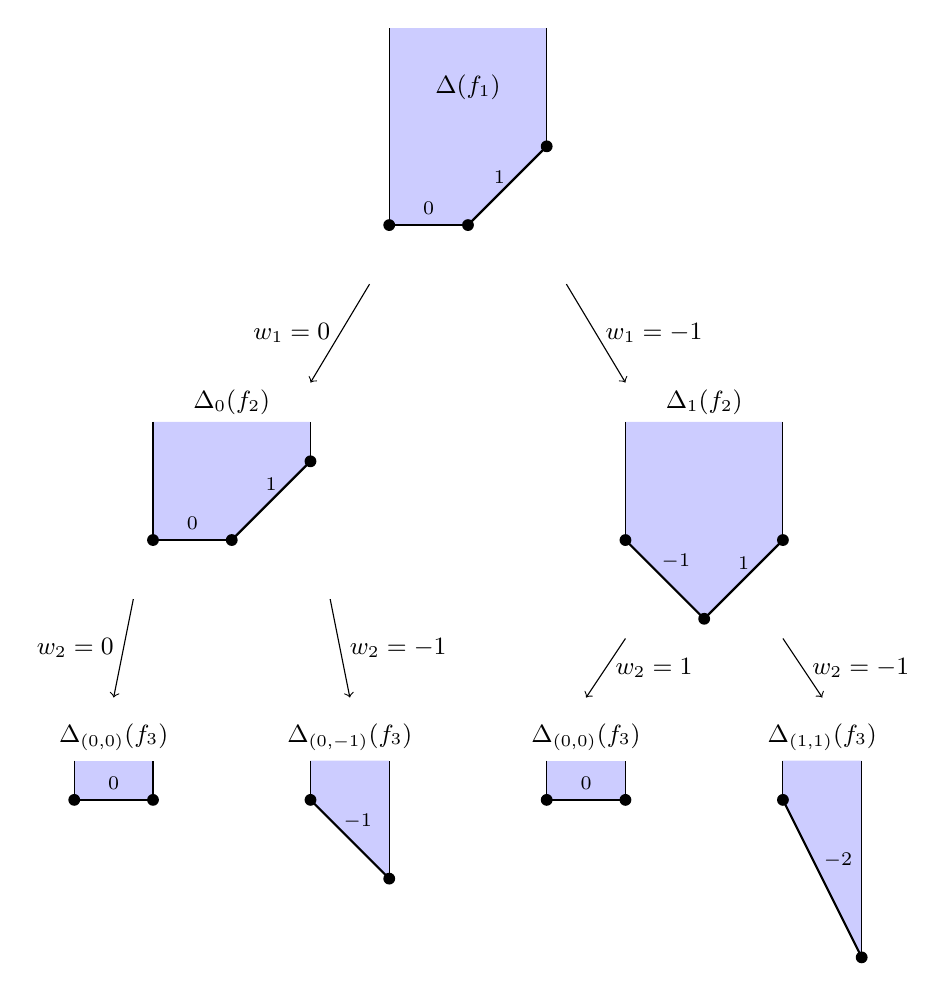
\begin{tikzpicture}
    % first level
    \fill[blue!20] (-1,2.5) -- (-1,0) -- (0,0) -- (1,1) -- (1,2.5) -- cycle;
    \draw (-1,2.5) -- (-1,0)
    (1,1) -- (1,2.5);
    \draw[thick,black]
      (-1,0) -- node[above,black,font=\scriptsize] {$0$} (0,0);
    \draw[thick,black]
      (0,0) -- node[anchor=south east,xshift=0.1cm,yshift=-0.1cm,black,font=\scriptsize] {$1$} (1,1);
    \fill (-1,0) circle (0.075cm);
    \fill (0,0) circle (0.075cm);
    \fill (1,1) circle (0.075cm);
    \node[font=\small] at (0,1.75) {$\Delta(f_1)$};

    \draw[->,black] (-1.25,-0.75) --
      node[left,black,font=\small] {$w_1=0$} ($(-1.25,-0.75)+(-0.75,-1.25)$);
    \draw[->,black] (1.25,-0.75) --
      node[right,black,font=\small] {$w_1=-1$} ($(1.25,-0.75)+(0.75,-1.25)$);

    % second level
    \node (o11) at (-3,-4) {};
    \fill[blue!20] ($(-1,1.5)+(o11)$) -- ($(-1,0)+(o11)$) -- ($(0,0)+(o11)$)
      -- ($(1,1)+(o11)$) -- ($(1,1.5)+(o11)$) -- cycle;
    \draw ($(-1,1.5)+(o11)$) -- ($(-1,0)+(o11)$)
      ($(1,1)+(o11)$) -- ($(1,1.5)+(o11)$);
    \draw[thick,black]
      ($(-1,0)+(o11)$) -- node[above,black,font=\scriptsize] {$0$} ($(0,0)+(o11)$);
    \draw[thick,black]
      ($(0,0)+(o11)$) -- node[above,black,font=\scriptsize] {$1$} ($(1,1)+(o11)$);
    \fill ($(-1,0)+(o11)$) circle (0.075cm);
    \fill ($(0,0)+(o11)$) circle (0.075cm);
    \fill ($(1,1)+(o11)$) circle (0.075cm);
    \node[font=\small] at ($(0,1.75)+(o11)$) {$\Delta_0(f_2)$};

    \draw[->,black] ($(-1.25,-0.75)+(o11)$) --
      node[left,black,font=\small] {$w_2=0$} ($(-1.25,-0.75)+(-0.25,-1.25)+(o11)$);
    \draw[->,black] ($(1.25,-0.75)+(o11)$) --
      node[right,black,font=\small] {$w_2=-1$} ($(1.25,-0.75)+(0.25,-1.25)+(o11)$);

    \node (o12) at (3,-4) {};
    \fill[blue!20] ($(-1,1.5)+(o12)$) -- ($(-1,0)+(o12)$) -- ($(0,-1) + (o12)$)
      -- ($(1,0)+(o12)$) -- ($(1,1.5)+(o12)$) -- cycle;
    \draw ($(-1,1.5)+(o12)$) -- ($(-1,0)+(o12)$)
      ($(1,0)+(o12)$) -- ($(1,1.5)+(o12)$);
    \draw[thick,black] ($(-1,0)+(o12)$) --
      node[above,black,font=\scriptsize,xshift=4pt] {$-1$} ($(0,-1)+(o12)$) --
      node[above,black,font=\scriptsize] {$1$} ($(1,0)+(o12)$);

    \fill ($(-1,0)+(o12)$) circle (0.075cm);
    \fill ($(0,-1)+(o12)$) circle (0.075cm);
    \fill ($(1,0)+(o12)$) circle (0.075cm);
    \node[font=\small] at ($(0,1.75)+(o12)$) {$\Delta_1(f_2)$};

    \draw[->,black] ($(-1,-1.25)+(o12)$) --
      node[right,black,font=\small] {$w_2= 1$} ($(-1.5,-0.75)+(0,-1.25)+(o12)$);
    \draw[->,black] ($(1,-1.25)+(o12)$) --
      node[right,black,font=\small] {$w_2= -1$} ($(1.5,-0.75)+(0,-1.25)+(o12)$);

    % third level
    \node (o21) at ($(o11)+(-2,-3.3)$) {};
    \fill[blue!20] ($(0,0.5)+(o21)$) -- ($(0,0)+(o21)$) -- ($(1,0)+(o21)$) -- ($(1,0.5)+(o21)$) -- cycle;
    \draw ($(0,0.5)+(o21)$) -- ($(0,0)+(o21)$)
      ($(1,0)+(o21)$) -- ($(1,0.5)+(o21)$);
    \draw[thick,black]
      ($(0,0)+(o21)$) -- node[above,black,font=\scriptsize] {$0$} ($(1,0)+(o21)$);
    \fill ($(0,0)+(o21)$) circle (0.075cm);
    \fill ($(1,0)+(o21)$) circle (0.075cm);
    \node[font=\small] at ($(0.5,0.8)+(o21)$) {$\Delta_{(0,0)}(f_3)$};

    \node (o22) at ($(o11)+(1,-3.3)$) {};
    \fill[blue!20] ($(0,0.5)+(o22)$) -- ($(0,0)+(o22)$) -- ($(1,-1)+(o22)$) -- ($(1,0.5)+(o22)$) -- cycle;
    \draw ($(0,0.5)+(o22)$) -- ($(0,0)+(o22)$)
      ($(1,-1)+(o22)$) -- ($(1,0.5)+(o22)$);
    \draw[thick,black]
      ($(0,0)+(o22)$) -- node[above,black,font=\scriptsize,xshift=0.1cm] {$-1$} ($(1,-1)+(o22)$);
    \fill ($(0,0)+(o22)$) circle (0.075cm);
    \fill ($(1,-1)+(o22)$) circle (0.075cm);
    \node[font=\small] at ($(0.5,0.8)+(o22)$) {$\Delta_{(0,-1)}(f_3)$};

    \node (o23) at ($(o12)+(-2,-3.3)$) {};
    \fill[blue!20] ($(0,0.5)+(o23)$) -- ($(0,0)+(o23)$) -- ($(1,0)+(o23)$) -- ($(1,0.5)+(o23)$) -- cycle;
    \draw ($(0,0.5)+(o23)$) -- ($(0,0)+(o23)$)
      ($(1,0)+(o23)$) -- ($(1,0.5)+(o23)$);
    \draw[thick,black]
      ($(0,0)+(o23)$) -- node[above,black,font=\scriptsize] {$0$} ($(1,0)+(o23)$);
    \fill ($(0,0)+(o23)$) circle (0.075cm);
    \fill ($(1,0)+(o23)$) circle (0.075cm);
    \node[font=\small] at ($(0.5,0.8)+(o23)$) {$\Delta_{(0,0)}(f_3)$};

    \node (o24) at ($(o12)+(1,-3.3)$) {};
    \fill[blue!20] ($(0,0.5)+(o24)$) -- ($(0,0)+(o24)$) -- ($(1,-2)+(o24)$) -- ($(1,0.5)+(o24)$) -- cycle;
    \draw ($(0,0.5)+(o24)$) -- ($(0,0)+(o24)$)
      ($(1,-2)+(o24)$) -- ($(1,0.5)+(o24)$);
    \draw[thick,black]
      ($(0,0)+(o24)$) -- node[above,black,xshift=0.2cm,font=\scriptsize] {$-2$} ($(1,-2)+(o24)$);
    \fill ($(0,0)+(o24)$) circle (0.075cm);
    \fill ($(1,-2)+(o24)$) circle (0.075cm);
    \node[font=\small] at ($(0.5,0.8)+(o24)$) {$\Delta_{(1,1)}(f_3)$};
  \end{tikzpicture}
  \caption{Series of Newton polygons of $F$ \cite[Figure~2]{tropPointsLinks}}
  \label{fig:seriesOfNewtonPolygons}
\end{figure}

With the ability to efficiently compute tropical varieties of zero-dimensional ideals we
can now focus on the central elements of fan traversals: Computing non-trivial points on a
tropical variety to find a starting cone and computing tropical links to determine
neighboring cones.

Finding non-trivial points on the tropical variety is achieved by intersecting with
sufficiently generic hyperplanes until the variety is zero-dimensional, allowing us to
apply Algorithm~\ref{alg:zeroDimTrop}. But when is a point non-trivial? For an ideal $I
\idealof K[\vec x]$ we define the \emph{homogeneity space} of $I$ to be the linear
subspace
\[
  C_0(I) = \left\{ \vec w \in \setR^n : \initial_{\vec w}(I) = I \right\}.
\]
It can be computed easily from any reduced Gröbner basis for $I$ and is trivially included
in $\Trop(I)$ if $I$ itself contains no monomial. In fact, $C_(I)$ is contained in every
cone of the tropical variety, so computing a point in the homogeneity space offers no
useful information for our algorithms. Hence, we call a point $\vec w \in \Trop(I)$
\emph{non-trivial}, if $\vec w \not\in C_0(I)$. The following proposition formalizes the
process of intersecting with generic hyperplanes:

\begin{proposition}
  Let $I \idealof K[\vec x]$ be an ideal of dimension $\dim I = d$ with algebraically
  independent set $\{x_1, \dots, x_d\}$ and suppose its affine variety $X := V(I)$
  satisfies $X \cap \setT^n \neq \varnothing$. Then there exists an non-empty Zariski-open
  subset $U \subseteq \setT^d$ such that for all $\lambda \in U$
  \[
    \varnothing \neq X_\lambda :=
    X \cap V(x_1-\lambda_1, \dots, x_d - \lambda_d) \subseteq \setT^n
  \]
  and $\dim X_\lambda = 0$.
  \label{prp:intersHyperp}
\end{proposition}

The resulting algorithm then just uses that the maximal cones in the tropical variety have
the same dimension as the defining ideal and puts Proposition~\ref{prp:intersHyperp} to
work:

\begin{algo}[Tropical Points, {\cite[Algorithm~3.3]{tropPointsLinks}}] $ $
  \begin{algorithmic}[1]
    \Require $I \idealof K[\vec x]$,
    \Ensure $\vec w \in \Trop(I) \setminus C_0(I)$.
    \State Compute a maximal algebraically independent set, say $\{x_1, \dots, x_d\}$ and
    the homogeneity space $C_0(I)$.
    \Repeat
      \State Pick $\vec w \in \setQ^d$ random with $\{\vec w\} \times \setR^{n-d} \cap
        C_0(I) = \varnothing$.
      \State Pick $c \in K^d$ random with $\nu(c) = \vec w$.
      \State Set $I_c := I|_{x_i = c_i} \idealof K[x_{d+1}, \dots, x_n]$
    \Until{$\dim(I_c) = 0$ and $V(I_c) \subseteq \setT^{n-d}$}
    \State Compute a triangular set $F$ with $I_c \subseteq \ideal F$.
    \State Compute $(w_{d+1}, \dots, w_n) \in \Trop(F)$ using
      Algorithm~\ref{alg:zeroDimTrop}.
    \State\textbf{return} $(w_1, \dots, w_d, w_{d+1}, \dots, w_n)$.
  \end{algorithmic}
  \label{alg:tropicalPoint}
\end{algo}

\begin{example}
  % TODO
  stuff
\end{example}

% TODO write differently from source?
Finally, to conclude this section we want study an alternative method of obtaining points
in neighboring cones. We call a tropical variety $\Trop(I)$ a \emph{tropical curve} if it
is one dimensional and say it is \emph{combinatorially a curve} if $\Trop(I)/C_0(I)$ is
one-dimensional. Then, for any $\vec u \in \Trop(I)$ sitting in the relative interior of a
cell of codimension one we call $\Trop(\initial_{\vec u}(I))$ the \emph{tropical link} of
$I$ around $\vec u$. This set is the support of a polyhedral fan, since it is a tropical
variety, and also combinatorially a curve which describes $\Trop(I)$ locally around $\vec
u$. The properties needed for our algorithm are as follows:

\begin{thmCorollary} \label{thmc:tropInt}
  Let $X$ and $X$ be two affine subvarieties. If the intersection $\Trop(X) \cap
  \Trop(X')$ has codimension $\codim\Trop(X) + \codim\Trop(X')$ in a neighborhood of $\vec
  w$, then $\vec w \in \Trop(X\cap X')$. In particular:
  \begin{enumerate}
    \item Assume $\Trop(I)$ is combinatorially a curve with $\dim C_0(I) = d$ and
      $C_0(I)\cap \Lin(e_{d+1}, \dots, e_n) = \{0\}$, then for any $c \in \setT^d$ we have
      \[
        \Trop(I) \cap \{\nu(c)\} \times \setR^{n-d} = \Trop(I + \ideal{x_1-c_1, \dots,
        x_d-c_d}),
      \]
      and this tropical variety is a tropical curve.
    \item If $\Trop(I)$ is a polyhedral fan, then for any $c \in K^*$ with
      $\nu(c)\neq0$ we have
      \[
        \Trop(I) \cap \{\nu(c)\} \times \setR^{n-1} = \Trop(I + \ideal{x_1-c_1})
      \]
      and this tropical variety is zero-dimensional.
  \end{enumerate}
\end{thmCorollary}

% TODO

\begin{algo}[Tropical Links, {\cite[Algorithm~4.5]{tropPointsLinks}}] $ $
  \begin{algorithmic}[1]
    \Require $I \idealof K[\vec x]$ such that $\Trop(I)$ is combinatorially a curve and a
    polyhedral fan,
    \Ensure $W \subseteq \setR^n$ such that $\Trop(I) = \bigcup_{\vec w \in W} \vec w
      \cdot \setR_{\geq0} + C_0(I)$
    \State Suppose $\dim C_0(I) = d$ and assume w.l.o.g. $C_0(I) \cap \Lin(e_{d+1}, \dots,
      e_n) = \{0\}$.
    \State Let $J \idealof K[x_d, \dots, x_n]$ be the image of $I$ under the substitution
      map
      \[
        K[x_1, \dots, x_n] \to K[x_d, \dots, x_n], x_i \mapsto
        \begin{cases}
          t, & \text{if } i < d, \\
          x_i & \text{else},
        \end{cases}
      \]
      where $t \in K$ is a fixed uniformizing parameter.
    \For{$i = d, \dots, n$}
      \State Let $J_i^\pm$ be the images of $J$ under the maps $x_i \mapsto t^\pm$
        respectively,
      \State Compute $V_i^\pm = \Trop(J_i^\pm)$ using Algorithm~\ref{alg:zeroDimTrop},
      \State Set
        \begin{align*}
          W_i^\pm := \Bigl\{
            &(1, \dots, 1, w_d, \dots, w_{i-1}, \pm1, w_{i+1}, \dots, w_n) : \\
            &(w_d, \dots, w_{i-1}, w_{i+1}, \dots, w_n) \in V_i^\pm
          \Bigr\} \subseteq \setR^n
        \end{align*}
      \State Scale elements of $W_i^\pm$ positively until they are primitive in $\setZ^n$.
    \EndFor
    \State Set $W = \bigcup_{i=d}^n (W_i^+ \cup W_i^-)$.
    \State\textbf{return} $W$.
  \end{algorithmic}
\end{algo}

This can then be used in Algorithm~\ref{alg:neighbors} as a replacement for line
\ref{alg:interiorPoints}.

\section{Parallelization}

Our main contribution is the combination of \textsc{Singular}-methods to compute tropical
varieties with recently developed parallelization efforts at the Fraunhofer ITWM of
computer algebra software. The first efforts to this end are described in
\cite{towardsParallel} while we specifically base our work on parallelization algorithms
by Christian Reinbold to compute GIT-fans (cite???). Parallelization of our procedures is
taken care of by the GPI-Space environment:

Use Petri nets as a framework to parallelize the traversal of tropical fans. Refer to
source \cite{towardsParallel}.

\subsection{Petri Nets}

Petri nets are used as a coordination language in GPI-Space, which allow us to formulate
our algorithms without explicitly specifying any parallelization. % TODO

\begin{definition}[Petri net]
  \label{def:petri}
  A \emph{Petri net} is a triple $N = (P, T, F)$ of two disjoint finite sets $P$ and $T$
  called \emph{places} and \emph{transitions} respectively and a subset $F \subseteq
  (P\times T) \cup (T \times P)$ called the \emph{flow relation} of the net.
\end{definition}

\subsection{GPI-Space}

Implementation with extensions

\subsection{Traversing a Fan in Parallel}
\label{sec:traverseParal}

Computing tropical varieties in our setting follows the general structure of a fan
traversal: Interpreting the maximal cones of a polyhedral fan together with their
adjacency relations as a connected graph, we may realize the fan traversal as a simple
graph traversal.

We formulate the traversal algorithm formulated in section~\ref{sec:tropVar} into a Petri
net.

Standard approach relying on a starting cone procedure and a \emph{neighbour oracle}.

\subsection{Existing Methods for Fan Traversals}

As previously mentioned we heavily rely on work done by Christian Reinbold on GIT-fans.
\dots

Introduce GIT-fans as similarly structured object

Adapting existing code base

\section{Performance and Scalability}

Benchmark speedup through parallelization.

Compute \enquote{big} examples to get a comparison.

\subsection{Tropical Grassmannians}

One important class of tropical varieties are the tropical Grassmannians which arise as
the tropical varieties of the equally -- if not more -- important Grassmannians which can
be interpreted as projective varieties. Some results on the tropical Grassmannian can be
found in \cite{tropGrass}.

\begin{definition}[Grassmannians]
  Let $n \in \setN_{>0}$ and $k \in \setN$ with $0 \leq k \leq n$, then the
  \emph{Grassmannian} of $k$-planes in $K^n$ is the set of all $k$-dimensional linear
  subspaces of $K^n$, usually denoted by $G(k, n)$.
\end{definition}

Thus, Grassmannians are in some sense a generalization of projective space: for instance
we will later be able to see that in fact $G(1,n) \cong \setP^n$. Our goal now is to give
these sets the structure of a projective variety which in turn allows us to study their
tropical variety. This is achieved by embedding a Grassmannian $G(k, n)$ into
$\setP^{\binom nk}-1$ via the so-called \emph{Plücker embedding}. To this end we want to
regard the corresponding linear spaces as elements of projective space, which first
requires some constructions from commutative algebra.

Let $V$ and $W$ be two vector spaces and $k\in\setN$, then a multilinear map $f : V^k \to
W$ is called \emph{alternating} if for all $v_1, \dots, v_k$ with $v_i=v_j$ for some
distinct $i,j$ we have that $f(v_1, \dots, v_k) = 0$. In this setting an \emph{alternating
$k$-fold tensor product} of $V$ is a vector space $T$ together with an alternating map
$\wedge:V^k\to T, (v_1, \dots, v_k) \mapsto v_1\wedge\cdots\wedge v_k$ such that for any
other alternating map $f:W\to T$ there is a unique $\tilde f:T\to W$ satisfying $\tilde f
\circ \wedge = f$. It is easy to prove that such an alternating tensor product always
exists and is in fact unique up to isomorphism -- the proof is completely analogous to the
case of standard tensor products. Hence we may write $\bigwedge^k V := T$ for these vector
spaces. In the following we present some interesting and necessary properties of these
spaces which can be proved with basic knowledge of commutative algebra:

\begin{remark}
  Let $V$ be a vector space, $k \in \setN$ and $\bigwedge^k V$ the corresponding
  alternating tensor product.
  \begin{enumerate}
    \item If $v_1, \dots, v_n$ is a basis of $V$ where $n=\dim V$ as a $K$-vector space,
      then the set
      \[
        \left\{
          v_{i_1} \wedge \cdots \wedge v_{i_k} : 1\leq i_1 < \cdots < i_k \leq n
        \right\}
      \]
      will be a basis of $\bigwedge^kV$. In particular this vector space is of dimension
      $\dim\bigwedge^kV = \binom nk$.
    \item For elements $v_1, \dots, v_k \in V$ the \emph{pure tensor} $v_1\wedge \cdots
      \wedge v_k \in \bigwedge^kV$ will be non-zero if and only if $v_1, \dots, v_k$ are
      linearly independent in $V$.
    \item It follows that for two linear independent families $v_1, \dots, v_k, w_1,
      \dots, w_k \in V$ we have that $v\wedge\cdots \wedge v_k$ and $w_1\wedge\cdots\wedge
      w_k$ are linearly dependent if and only if the families both span the same linear
      subspace of $V$.
  \end{enumerate}
\end{remark}

Consider now our setting where $V=K^n$ and let $N = \binom nk$ be the number of basis
elements in $\bigwedge^kK^n$. We may identify a $k$-dimensional linear subspace $X \in
G(k,n)$ of $V$ with a pure tensor in $\bigwedge^kV \cong K^N$ uniquely up to scalar
multiplication which -- by definition -- makes the corresponding embedding $G(k,n) \to
\setP^{N-1}$, called the \emph{Plücker embedding}, injective. Hence we can regard $G(k,n)$
as a subset of this projective space. Finally, to equip $G(k,n)$ with the structure of a
projective variety, we need this fact: For non-zero $w\in \bigwedge^kK^n$ the rank of the
$K$-linear map $f:K^n \to \bigwedge^{k+1}K^n, v \mapsto v \wedge w$ is at least $n-k$ and
equality holds if and only if $w$ is a pure tensor. Thus, using the above embedding,
$G(k,n)$ consists entirely of pure tensors $w\in G(k,n)$ which all define maps $v\mapsto
v\wedge w$ of rank at most $n-k$. This is equivalent to all $(n-k+1) \times
(n-k+1)$-minors of these maps vanishing which induces polynomial equations in the Plücker
coordinates of $\setP^{N-1}$ describing $G(k,n)$, hence it is in fact a projective
variety.

On an additional note one can cover $G(k,n)$ with copies of $\setA^{k(n-k)}$ to show that
the Grassmannian is an irreducible projective variety of dimension $k(n-k)$. This leads to
the following definition:

\begin{definition}[Tropical Grassmannians]
  By the above a Grassmannian can be viewed as a projective variety given by a homogeneous
  ideal
  \[
    I(G(k,n)) \idealof K[ p_{i_1, \dots, i_k} : 1\leq i_1 < \cdots < i_k \leq n ]
  \]
  with Plücker coordinates $p_{i_1,\dots,i_k}$ which defines a determinantal variety $G(k,
  n)$. This, in turn, defines a tropical variety and we write $\mathcal G_{k,n} :=
  \Trop(I(G(k,n)))$.
\end{definition}

\subsection{Runtime Measurements}

\begin{figure}[htbp]
  \begin{center}
    \input{fig/scaling.tex}
  \end{center}
  \caption{Running times of computing $\mathcal{G}_{3,8}$}
  \label{fig:g38scaling}
\end{figure}

In figure~\ref{fig:g38scaling} we see that \dots and so on.

\begin{figure}[htbp]
  \begin{center}
    \input{fig/efficiency.tex}
  \end{center}
  \caption{Parallelization efficiency of computing $\mathcal{G}_{3,8}$}
  \label{fig:g38efficiency}
\end{figure}

\subsection{Practical Optimizations}

Optimization of certain edge cases

Mention improvements to \textsc{Singular} kernel here?

\newpage
\listoffigures
\newpage% only maybe
\printbibliography

\end{document}
% vim: spell spelllang=en
